\section{Einstieg}

\begin{frame}{Problemstellung}
	\begin{itemize}
		\item Punkte gleichmäßig im Raum verteilen
		\item<3-> Mehrere existierende Verfahren
		\begin{itemize}
			\item<4-> Halton
			\item<4-> Blue noise
		\end{itemize}
		\item<5-> \textbf{Ziel}: effizientes Vorgehen 
	\end{itemize}
	\begin{figure}
		\begin{subfigure}{.3\textwidth}
			\centering
			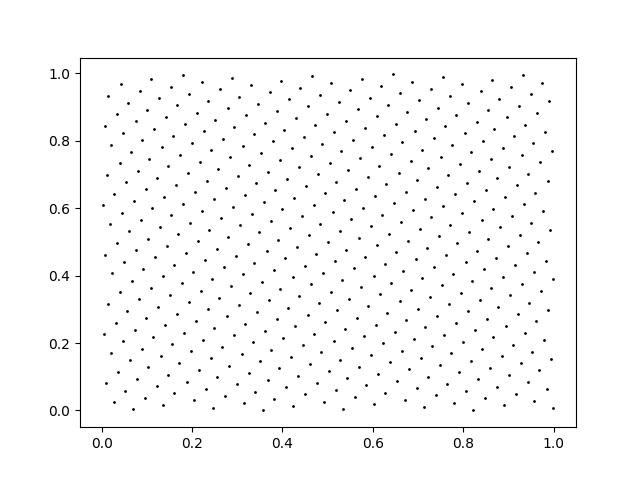
\includegraphics[width=\textwidth]{pdf_plots/grs_u500c.pdf}<2->
		\end{subfigure}
		\hfill
		\begin{subfigure}{.3\textwidth}
			\centering
			
\includegraphics[width=.5\textwidth, angle=180]{Screenshots/img_71815.png}<2->
		\end{subfigure}
		\begin{subfigure}{.3\textwidth}
			\centering
			\includegraphics[width=\textwidth]{pdf_plots/idf2_log-log_iu500c-GRS.pdf}<2->
		\end{subfigure}
	\end{figure}
\end{frame}